\chapter{Análise Estatística Não Paramétrica}
\label{chap:analise_estatistica_np}
Considerando que as distribuições das métricas de conectividade (diferença entre Pós e Pré) não se comportam de maneira normal (ver Capítulo~\ref{chap:analise_distribuicao_normalidade}), optamos por empregar testes estatísticos não paramétricos para comparar as condições de estimulação \textit{cathodic} versus \textit{sham}. Essa escolha evita pressupostos inadequados sobre a distribuição dos dados. Além da violação de normalidade, a presença de \texit{outliers} reforça a adoção de testes não paramétricos neste cenário de heterogeneidade amostral.

Nesta etapa, foram aplicados os seguintes testes estatísticos não paramétricos:

\begin{itemize}
    \item \textbf{\textit{Mann-Whitney U}:} Teste para amostras independentes, usado para avaliar se a distribuição das diferenças entre as condições difere significativamente entre os grupos. O tamanho do efeito foi estimado com base na estatística U e no número de observações em cada condição.
    
    \item \textbf{\textit{Wilcoxon signed-rank}:} Teste para amostras pareadas, que compara os valores dentro de cada participante, canal e faixa de frequência, permitindo avaliar mudanças intraindividuais entre as condições.

    \item \textbf{\textit{Kruskal-Wallis}:} Teste para múltiplos grupos, empregado para verificar diferenças globais ao longo das faixas de frequência. A significância indica se pelo menos uma das bandas se comporta de forma distinta, sem especificar quais.
\end{itemize}

Os testes foram realizados separadamente para cada uma das métricas de conectividade (\texttt{median\_plv\_diff}, \texttt{median\_pli\_diff} e \texttt{median\_cf\_plm\_diff}) e para os dois grupos de canais: \texttt{EEG\_EEG} e \texttt{EEG\_ECG}. Ressalta-se que, embora o código inclua procedimentos para remoção de dados nulos, na prática esses valores não estão presentes, servindo apenas para tratamento de exceções.

\section{Resultados dos Testes}
Nesta seção, comparamos as diferenças (pós -- pré) das métricas de conectividade entre as condições \textit{cathodic} e \textit{sham} por meio de três testes não-paramétricos: \textit{Mann-Whitney U}, \textit{Wilcoxon signed-rank} e \textit{Kruskal-Wallis}. Cada teste fornece uma perspectiva ligeiramente distinta sobre as diferenças entre os grupos de dados:

\begin{itemize}
  \item \textbf{\textit{Mann-Whitney U} (amostras independentes):} Avalia se as distribuições da métrica em \textit{cathodic} e \textit{sham} diferem de forma consistente em seus valores medianos, quando os grupos não são necessariamente pareados.
  \item \textbf{\textit{Wilcoxon signed-rank} (amostras pareadas):} Verifica se há diferença na mesma variável entre dois estados para o \emph{mesmo} participante ou canal, isto é, um teste de antes e depois (pós -- pré) que controla variações intraindividuais.
  \item \textbf{\textit{Kruskal-Wallis} (comparação de múltiplos grupos):} Geralmente utilizado para verificar se há diferença \emph{global} entre três ou mais grupos, mas aqui também se aplica a subdivisões (como faixas de frequência) para avaliar se alguma banda difere significativamente das demais.
\end{itemize}

\subsection{Métricas para \texttt{median\_pli\_diff}}

\paragraph{Grupo EEG\_EEG:}
\begin{itemize}
    \item \textbf{\textit{Mann-Whitney U}:} As faixas \emph{alpha}, \emph{delta}, \emph{gamma} e \emph{theta} exibiram diferenças estatisticamente significativas (p-valores $< 0.001$) entre \emph{cathodic} e \textit{sham}. Já a faixa \emph{beta} teve um resultado marginal ($p \approx 0.051$), sugerindo uma possível tendência à diferença, mas não alcançando significância pelo critério habitual ($\alpha=0.05$).
    \item \textbf{\textit{Wilcoxon}:} Ao tratar cada participante (ou par de canais) como pareado, observamos que todas as bandas apresentaram p-valores muito baixos, com tamanho de efeito em torno de $0.477$. Isso reforça a ideia de que, na maior parte das faixas de frequência, há uma mudança consistente entre pré e pós, distinta para \textit{cathodic} vs. \textit{sham}.
    \item \textbf{\textit{Kruskal-Wallis}:} Novamente, \emph{alpha}, \emph{delta}, \emph{gamma} e \emph{theta} demonstraram diferenças significativas na comparação global. A \emph{beta} foi marginal, o que sugere que, ao analisar globalmente as bandas, \emph{beta} não se destacou tanto.
\end{itemize}

\paragraph{Interpretação:}
Os resultados indicam que a \texttt{median\_pli\_diff} (EEG-EEG) sofre mudanças significativas na maior parte das faixas de frequência, seja considerando grupos independentes (\textit{Mann-Whitney U}), seja observando pares de medidas para cada sujeito/canal (\textit{Wilcoxon}). Já o \textit{Kruskal-Wallis}, que avalia diferenças globais entre bandas, mostra que \emph{alpha}, \emph{delta}, \emph{gamma} e \emph{theta} se destacam de forma consistente, enquanto \emph{beta} está no limite de significância. 
Na prática, isso sugere que a estimulação catódica influencia de modo mais evidente a sincronização nessas quatro bandas em comparação à \emph{beta}. Ademais, em faixas como \emph{alpha}, \emph{delta} e \emph{theta}, o \emph{effect size} geralmente aponta para valores mais elevados de \emph{PLI} sob \textit{cathodic}, indicando um provável aumento na sincronia de fase frente ao \textit{sham}.

\subsection{Métricas para \texttt{median\_cf\_plm\_diff}}
\paragraph{Grupo EEG\_ECG:}
\begin{itemize}
    \item \textbf{\textit{Mann-Whitney U}:} As faixas \emph{alpha}, \emph{beta} e \emph{delta} apresentaram diferenças significativas (p-valores $< 0.05$), enquanto \emph{gamma} e \emph{theta} não mostraram significância estatística.
    \item \textbf{\textit{Wilcoxon}:} Todos os testes resultaram em p-valores muito baixos, com tamanhos de efeito em torno de 0.358, indicando um efeito consistente de \textit{cathodic} vs. \textit{sham} quando avaliado \emph{intra-sujeito/canal}.
    \item \textbf{\textit{Kruskal-Wallis}:} As bandas \emph{alpha}, \emph{beta} e \emph{gamma} revelaram diferenças na análise global, mas \emph{delta} e \emph{theta} não se destacaram nesse critério.
\end{itemize}

\paragraph{Interpretação:}

No caso da \texttt{median\_cf\_plm\_diff} (EEG-ECG), encontramos resultados que divergem ligeiramente conforme o teste aplicado: enquanto \textit{Mann-Whitney U} e \textit{Wilcoxon} apontam a significância de \textit{alpha}, \textit{beta} e \textit{delta}, o \textit{Kruskal-Wallis} identifica \textit{gamma}, porém não confirma \textit{delta} e \textit{theta}. Isso reflete a menor sensibilidade do teste global (\textit{Kruskal-Wallis}) para certas diferenças pontuais, bem como a possível variabilidade nos pares EEG-ECG. De forma geral, \textit{alpha} e \textit{beta} exibem valores \texttt{cf\_plm\_diff} mais elevados na condição \textit{cathodic}, indicando maior sincronicidade EEG-ECG após a estimulação catódica em comparação à condição \textit{sham}


\subsection{Conclusão Geral dos Testes}
Em síntese, os três testes não-paramétricos evidenciam mudanças estatisticamente significativas nas métricas \texttt{median\_pli\_diff} e \texttt{median\_cf\_plm\_diff}, abrangendo várias faixas de frequência. Cada teste ressalta um aspecto distinto:
\begin{itemize}
    \item \textit{Mann-Whitney U}: Indica diferenças globais entre \textit{cathodic} e \textit{sham}.
    \item \textit{Wilcoxon}: Reforça as mudanças intraindividuais (pós--pré), sinalizando consistência dos efeitos.
    \item \textit{Kruskal-Wallis}: Mostra variações no espectro como um todo, apontando quais faixas são mais afetadas.
\end{itemize}

Esses achados, em conjunto, corroboram a hipótese de que a neuromodulação catódica sobre o DLPFC impacta os padrões de sincronização em \textit{resting-state}, tanto no PPC \textit{same-frequency} EEG-EEG quanto no PPC \textit{cross-frequency} EEG-ECG. A consistência entre testes diferentes aumenta a confiança de que os efeitos observados não são atribuíveis a ruídos ou a variações aleatórias.

\section{Discussão e Justificativa dos Métodos}
Os testes de normalidade indicaram violações significativas dos pressupostos de normalidade para as métricas de conectividade analisadas, o que justificou o uso de testes não paramétricos para comparar as condições de estimulação (\texttt{\textit{cathodic}} versus \texttt{\textit{sham}}). Esses métodos não dependem de pressupostos sobre a distribuição dos dados.

A aplicação conjunta de múltiplos testes (\textit{Mann-Whitney U}, \textit{Wilcoxon} e \textit{Kruskal-Wallis}) permitiu uma avaliação abrangente das diferenças entre as condições, considerando tanto comparações entre grupos independentes quanto análises pareadas intraindividuais. Os resultados indicam que, para a maioria das faixas de frequência e para as métricas \texttt{median\_pli\_diff} e \texttt{median\_cf\_plm\_diff}, existem diferenças estatisticamente significativas entre as condições, reforçando a importância da modulação induzida pela estimulação.

Por outro lado, os achados para as métricas de sincronização, em especial no contexto EEG–ECG, exibiram variações dependendo do teste estatístico e da faixa de frequência considerada. Esse fato indica que cada método (Mann–Whitney, \textit{Wilcoxon} ou Kruskal–Wallis) pode captar aspectos distintos dos dados ou apresentar sensibilidades diferentes à variabilidade intra e intersujeitos.

\section{Detecção de \textit{Outliers}, Análise \textit{Bootstrap} e Correções para Comparações Múltiplas}
Para avaliar o impacto dos pontos atípicos nas análises subsequentes, optamos por realizar uma etapa adicional de detecção e remoção de \texit{outliers} utilizando o método ECOD, especialmente adequado ao nosso conjunto de dados devido à sua natureza não paramétrica, identificando anomalias sem pressupor uma distribuição específica dos dados. Estudos demonstram que o ECOD supera diversas técnicas convencionais de detecção de \texit{outliers} em termos de acurácia e eficiência \cite{li2022ecod}.

Aplicamos o ECOD considerando as métricas \texttt{median\_pli\_diff} e \texttt{median\_cf\_plm\_diff}. Inicialmente, o dataset continha 122915 entradas; após a aplicação do ECOD, aproximadamente 5,00\% dos dados foram identificados como \texit{outliers} e removidos.

Posteriormente, implementamos um pipeline de análise baseado em \textit{Bootstrap} acelerado por placa de vídeo (GPU) para o cálculo de intervalos de confiança \textit{Bias-Corrected and Accelerated} (BCa). Esse método é particularmente robusto, pois ajusta tanto o viés quanto a aceleração da distribuição \textit{Bootstrap}, permitindo capturar assimetrias e a influência residual de \texit{outliers} nos dados. Embora computacionalmente custoso, o método BCa é amplamente reconhecido como uma das abordagens mais precisas para a estimação de intervalos de confiança em situações onde os pressupostos de normalidade não são atendidos. Optamos por esse método em detrimento de outras técnicas devido à sua capacidade de corrigir distorções na distribuição da estatística estimada.

Para avaliar a significância estatística após múltiplas comparações, utilizamos a função \texttt{multipletests} da biblioteca Python \texttt{statsmodels} com o método \textit{Bonferroni}. Este procedimento ajusta os p-valores originais multiplicando-os pelo número total de comparações realizadas, tornando o critério de significância mais conservador e minimizando o risco de falsos positivos. Dessa forma, efeitos são considerados significativos quando o p-valor corrigido por \textit{Bonferroni} for inferior a 0,05.

Além disso, nosso pipeline incluiu o cálculo de tamanhos de efeito utilizando diversas métricas, tais como:
\begin{itemize}
    \item \textbf{\textit{Cohen's d}} e \textbf{\textit{Hedges' g}}: que quantificam a magnitude da diferença entre as condições em termos de desvios-padrão;
    \item \textbf{\textit{Rank-Biserial Correlation} (RBC)}: derivado do teste de \textit{Wilcoxon}, que fornece uma interpretação robusta baseada em postos.
\end{itemize}

Essas métricas complementares permitem uma avaliação abrangente do efeito da estimulação e possibilitam comparar os resultados obtidos com diferentes abordagens, como o método de \textit{Bonferroni}, Holm e \textit{False Discovery Rate-Benjamini–Hochberg} (FDR-BH), fornecendo uma visão mais robusta e diversificada dos achados.

Em resumo, nossa abordagem compreende as seguintes etapas:
\begin{enumerate}
    \item \textbf{Detecção de \textit{Outliers}:} Utilizamos o método ECOD para identificar e remover aproximadamente 5\% dos dados considerados anômalos, garantindo a robustez das análises.
    \item \textbf{Análise \textit{Bootstrap} com GPU:} Implementamos o cálculo de intervalos de confiança BCa, estimando viés, erro padrão e tamanhos de efeito por meio de reamostragem acelerada, assegurando precisão mesmo em distribuições assimétricas.
    \item \textbf{Testes Não Paramétricos e Correção para Comparações Múltiplas:} Aplicamos testes não paramétricos, como o teste de \textit{Wilcoxon} para dados emparelhados, e corrigimos os p-valores utilizando o método \textit{Bonferroni} (além de outras correções complementares), minimizando o risco de erros do tipo I.
\end{enumerate}

Os resultados deste processamento serão apresentados em detalhes nos anexos, permitindo a comparação dos resultados obtidos com e sem a remoção de \texit{outliers}, bem como a análise dos diferentes tamanhos de efeito e métodos de correção.

\section{Distribuição de Tamanhos de Efeito e p-valores}
\label{sec:effect_size_distribution}
Nesta etapa, examinamos a distribuição das estimativas de tamanho de efeito (\textit{Cohen's d}, \textit{Hedges' g} e \textit{Wilcoxon RBC}) e dos valores-p (brutos e corrigidos por \textit{Bonferroni}) para as análises de PLI (EEG-EEG) e CF-PLM (EEG-ECG), considerando cenários com e sem \texit{outliers}. A Figura~\ref{fig:effectsizehist_all} ilustra, em quatro subfiguras, como essas métricas se distribuem ao longo dos pares de canal e faixas de frequência analisados.

\begin{figure}[htb]
    \centering
    % Subfigura 1: PLI (EEG-EEG), Sem Outliers
    \subfloat[Sem Outliers -- PLI (EEG-EEG)]{
        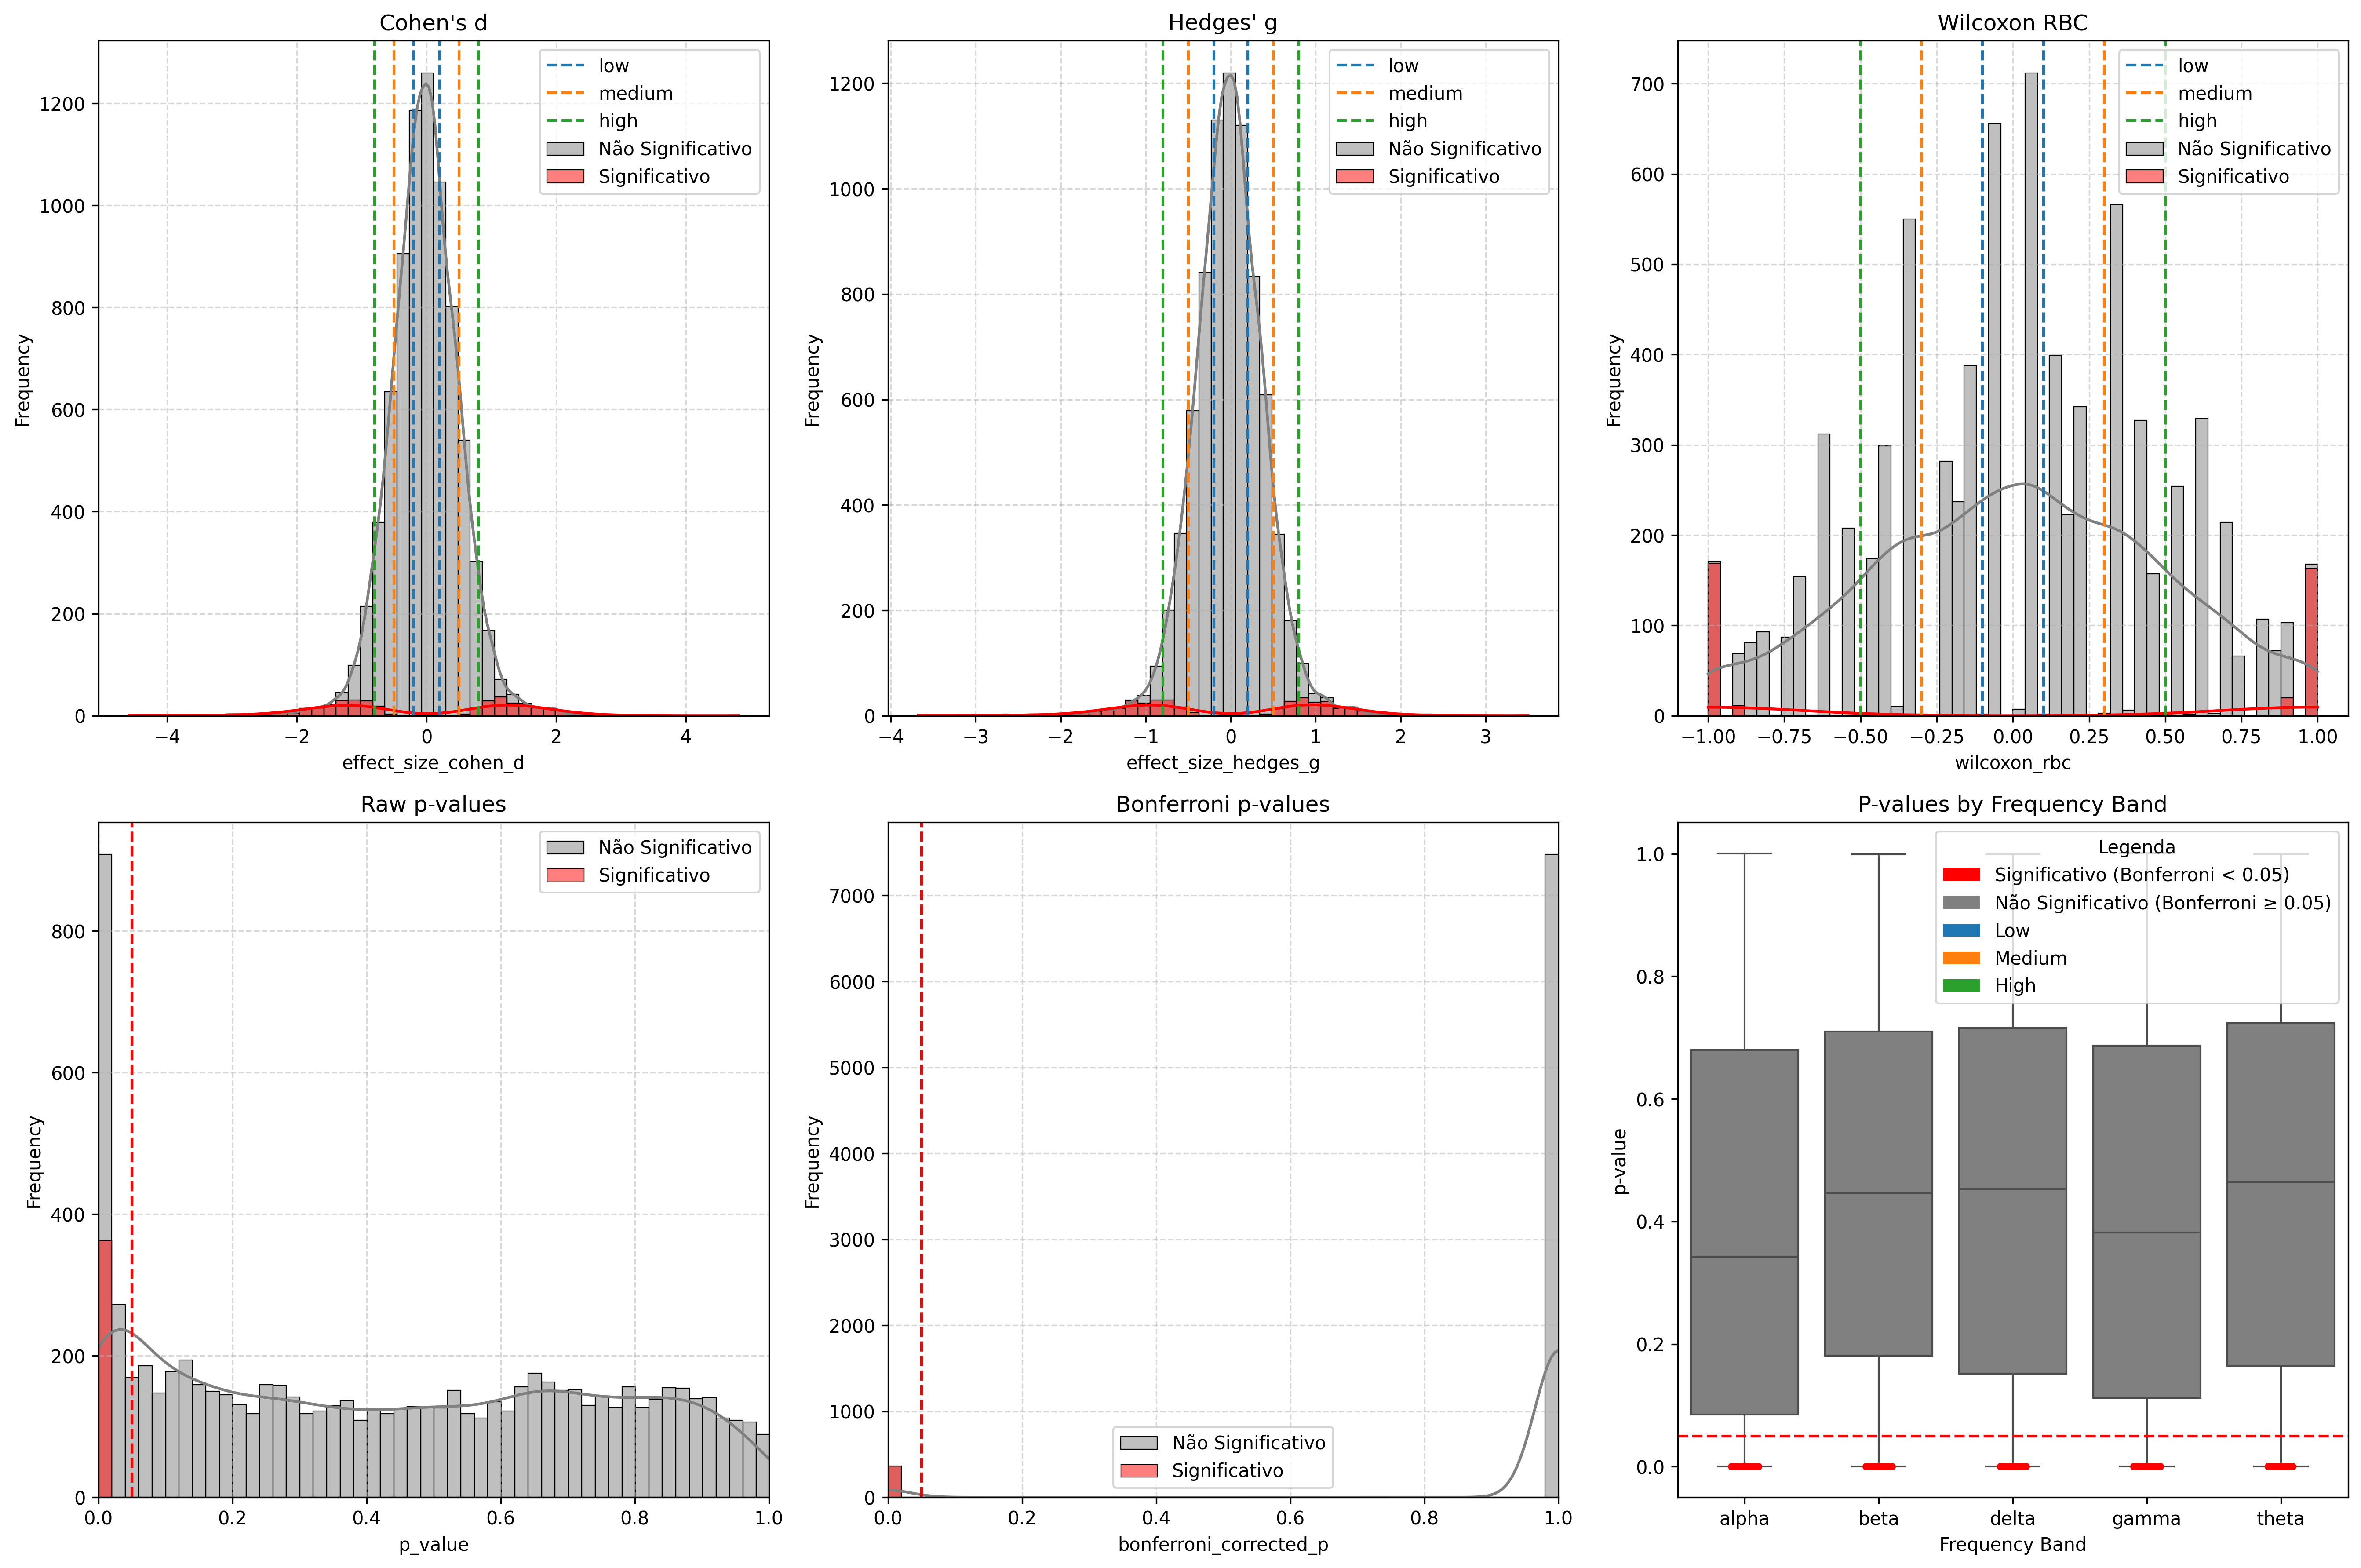
\includegraphics[width=0.45\textwidth]{figs/7_bootstrap_results_analysis/1_effect_size_histograms/Effect_Size_Histograms_PLI_EEGEEG_Sem_Outliers.png}
    }
    \quad
    % Subfigura 2: CF-PLM (EEG-ECG), Sem Outliers
    \subfloat[Sem Outliers -- CF-PLM (EEG-ECG)]{
        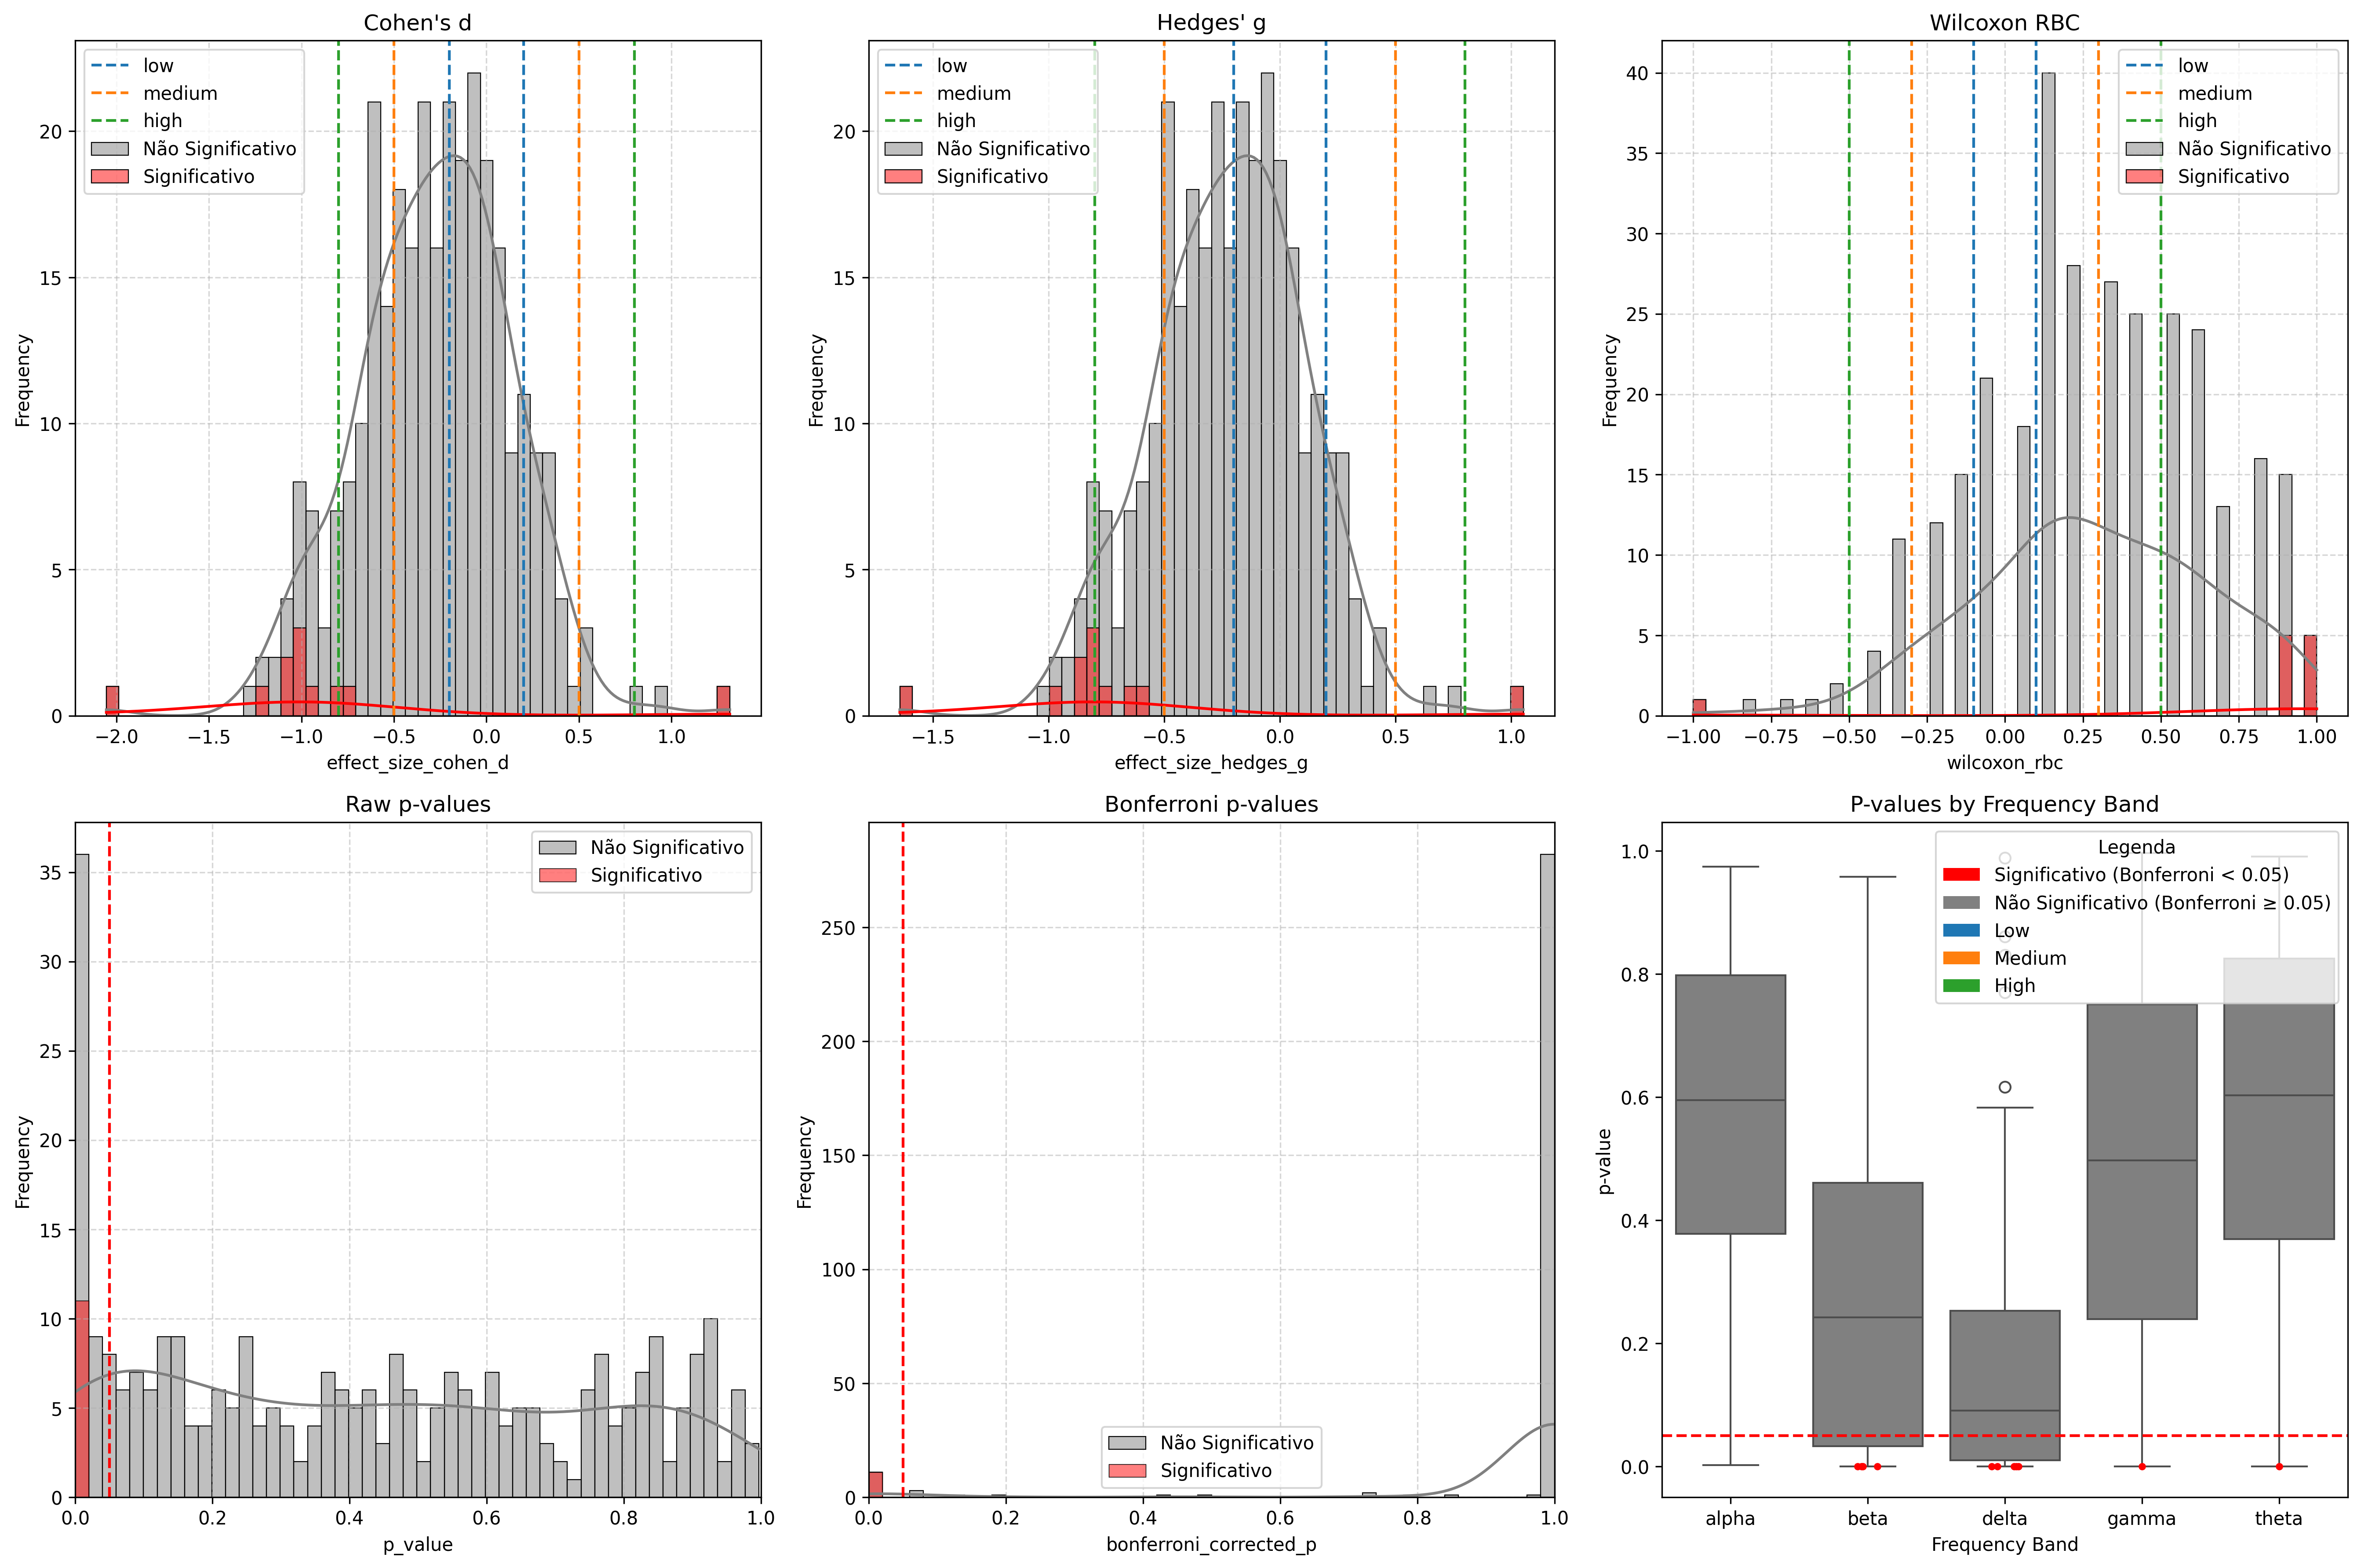
\includegraphics[width=0.45\textwidth]{figs/7_bootstrap_results_analysis/1_effect_size_histograms/Effect_Size_Histograms_CFPLM_EEGECG_Sem_Outliers.png}
    }
    \\
    % Subfigura 3: PLI (EEG-EEG), Com Outliers
    \subfloat[Com Outliers -- PLI (EEG-EEG)]{
        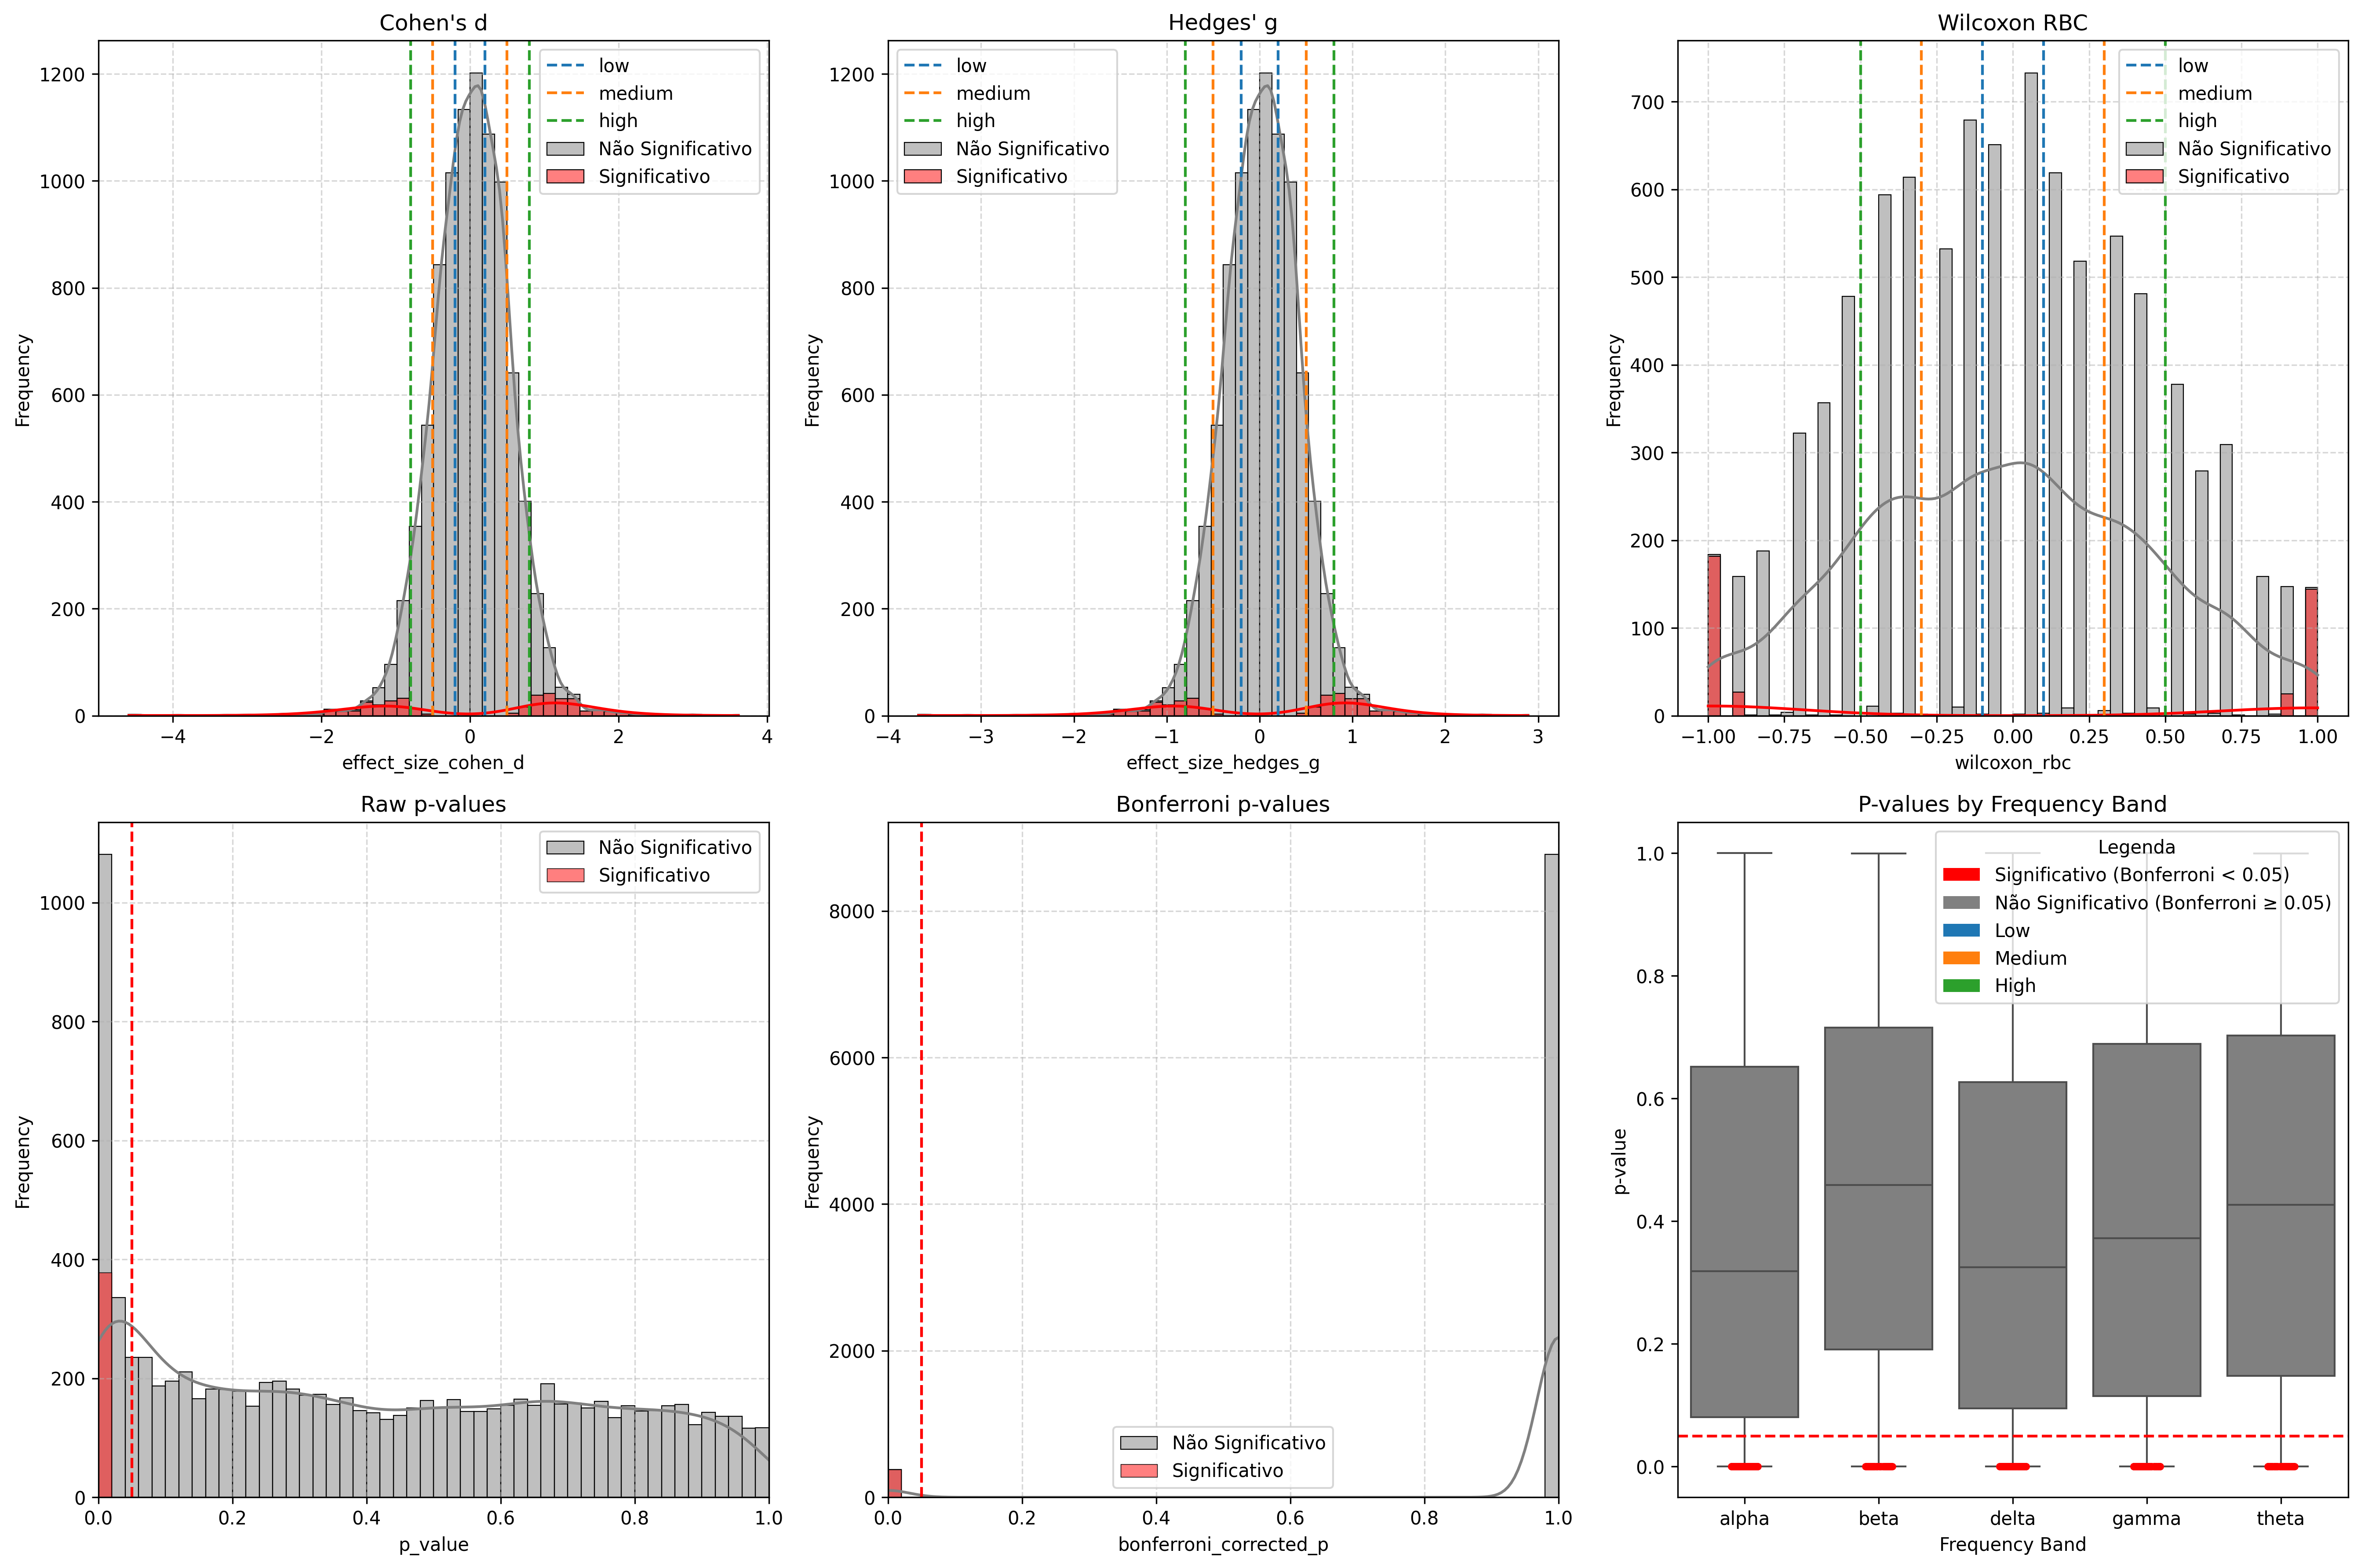
\includegraphics[width=0.45\textwidth]{figs/7_bootstrap_results_analysis/1_effect_size_histograms/Effect_Size_Histograms_PLI_EEGEEG_Com_Outliers.png}
    }
    \quad
    % Subfigura 4: CF-PLM (EEG-ECG), Com Outliers
    \subfloat[Com Outliers -- CF-PLM (EEG-ECG)]{
        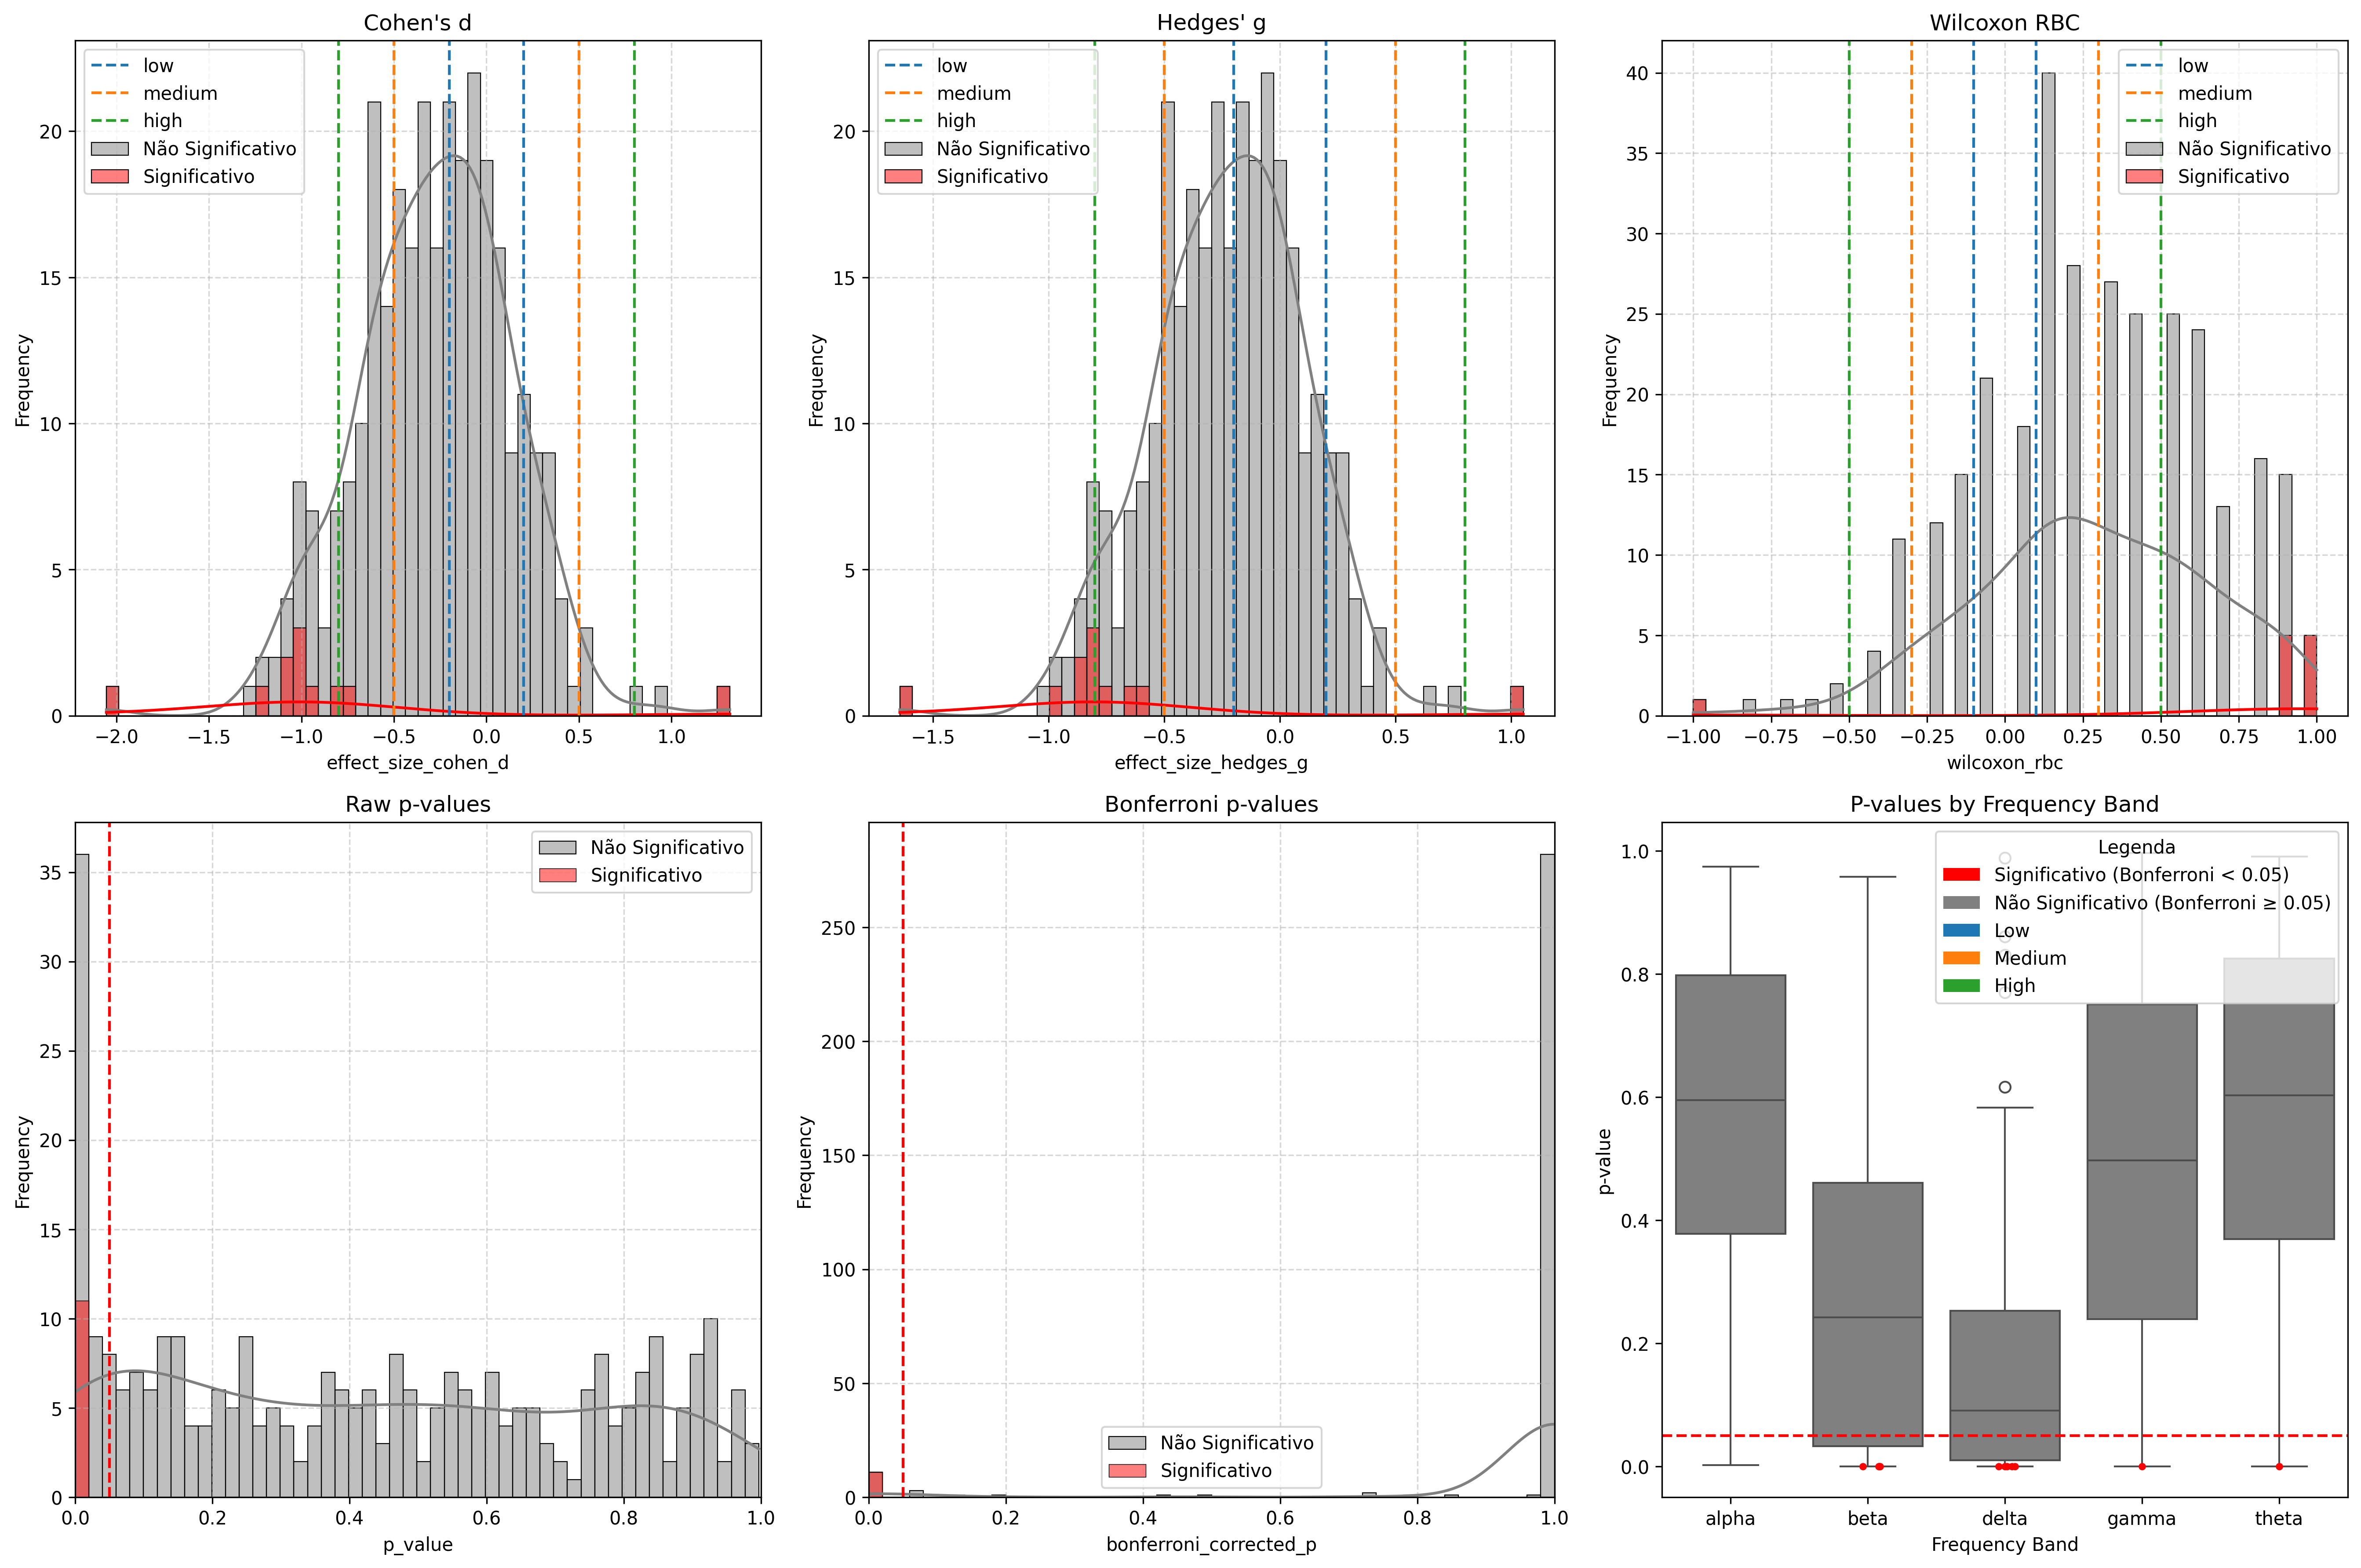
\includegraphics[width=0.45\textwidth]{figs/7_bootstrap_results_analysis/1_effect_size_histograms/Effect_Size_Histograms_CFPLM_EEGECG_Com_Outliers.png}
    }
    \caption[Distribuições de tamanhos de efeito e valores-p]{Distribuição das métricas de tamanho de efeito (\textit{Cohen's d}, \textit{Hedges' g} e \textit{Wilcoxon RBC}) e dos valores-p (brutos e corrigidos por \textit{Bonferroni}) para PLI (EEG-EEG) e CF-PLM (EEG-ECG), em cenários com e sem \texit{outliers}. O \textit{Wilcoxon RBC} e o p-valor corrigido por \textit{Bonferroni} (vertical tracejada vermelha em $p=0.05$) foram escolhidos como as métricas para representar, respectivamente, o tamanho do efeito e a significância estatística nas análises subsequentes.}
    \label{fig:effectsizehist_all}    
\end{figure}

\subsection{Distribuição dos Tamanhos de Efeito}
\paragraph{\textit{Cohen's d} e \textit{Hedges' g}}
\begin{itemize}
    \item A maior parte dos valores concentra-se em torno de zero, indicando que, para a maioria dos pares, as diferenças entre as condições \textit{cathodic} e \textit{sham} são pequenas ou não significativas.
    \item Valores significativos (representados pelas barras vermelhas nos histogramas) tendem a se afastar de zero, sinalizando diferenças mais acentuadas. Por exemplo, valores de \textit{Cohen's d} ou \textit{Hedges' g} superiores a 0.5 (ou inferiores a -0.5) sugerem um efeito moderado, enquanto valores acima de 0.8 (ou inferiores a -0.8) indicam um efeito alto.
    \item Embora \textit{Hedges' g} difira de \textit{Cohen's d} ao aplicar uma correção para tamanhos amostrais pequenos, ambas as métricas exibem comportamentos semelhantes nos histogramas.
\end{itemize}

\paragraph{\textit{Wilcoxon Rank-Biserial Correlation} (\textit{Wilcoxon RBC})}
\begin{itemize}
    \item O \textit{Wilcoxon RBC} é derivado do teste não paramétrico de \textit{Wilcoxon} e reflete a correlação de postos entre as condições, tipicamente variando de -1 a +1.
    \item Por não exigir pressupostos de normalidade, o RBC se mostra mais robusto no tratamento de dados heterogêneos e na presença de \texit{outliers}.
    \item Valores acima de 0.3 ou abaixo de -0.3 sugerem um efeito moderado; valores acima de 0.5 (ou abaixo de -0.5) indicam um efeito alto, e quando se aproximam de ±1, as condições diferem de forma quase absoluta.
    \item Devido a essa robustez, o RBC foi escolhido como nosso principal indicador de tamanho de efeito nas análises subsequentes.
\end{itemize}

\subsection{Distribuição de p-valores (Brutos e Corrigidos)}
\begin{itemize}
    \item Os histogramas de p-valores brutos mostram uma forte concentração em torno de 1 (indicando resultados não significativos) e uma cauda próxima de 0 (sinalizando potenciais resultados significativos).
    \item Após a correção de \textit{Bonferroni} (indicada pela linha vertical tracejada em \(p=0.05\)), muitos dos valores que eram marginalmente significativos foram deslocados para a região de não significância, evidenciando o caráter conservador deste método de correção.
    \item Devido ao elevado número de comparações, a utilização do método \textit{Bonferroni} minimiza a probabilidade de falsos positivos, sendo adotado como critério principal para a significância estatística.
\end{itemize}

\subsection{Comparação Entre Cenários (Com e Sem Outliers)}
\begin{itemize}
    \item \textbf{Impacto da Remoção de \textit{Outliers}:} De modo geral, a remoção de \texit{outliers} reduz ligeiramente o número de casos significativos em EEG-EEG, mas não altera substancialmente a distribuição dos tamanhos de efeito ou dos p-valores. No caso do EEG-ECG, a diferença entre manter ou remover \texit{outliers} é mínima, indicando que a presença de valores extremos tem pouco impacto na detecção de efeitos significativos nesse grupo.

    \item \textbf{PLI (EEG-EEG):} O número de comparações realizadas no cenário EEG-EEG é consideravelmente maior, pois cada um dos 61 canais de EEG forma pares com os demais canais EEG. Isso resulta em \( 61 \times 60 \) pares únicos por banda de frequência. Com 5 bandas de frequência e 6 atletas, obtemos um total de aproximadamente \( 109.800 \) comparações. Entre essas, foram identificados entre \( 363 \) (com remoção de \texit{outliers}) e \( 378 \) (sem remoção de \texit{outliers}) casos significativos.

    \item \textbf{CF-PLM (EEG-ECG):} Em contraste, no cenário EEG-ECG, cada um dos 61 canais EEG é comparado a um único canal de ECG, resultando em \( 61 \times 1 \) pares por banda de frequência. Assim, considerando as mesmas 5 bandas e 6 atletas, temos um total de \( 3.660 \) comparações, o que representa uma redução drástica na quantidade de testes estatísticos realizados em relação ao EEG-EEG. Como esperado, isso levou à detecção de um número muito menor de casos significativos, totalizando apenas \( 11 \).

    \item \textbf{Robustez do RBC e do \textit{Bonferroni}:} Independentemente da remoção de \texit{outliers}, as comparações que apresentam valores elevados de \textit{Wilcoxon RBC} e p-valores corrigidos abaixo de \( 0.05 \) permanecem confiáveis. Isso reforça a utilidade dessas métricas como principais indicadores da magnitude e significância estatística dos efeitos encontrados, independentemente da heterogeneidade dos dados.
\end{itemize}

Em resumo, os histogramas de \textit{Wilcoxon RBC} (indicador de tamanho de efeito) e os p-valores corrigidos por \textit{Bonferroni} (indicador de significância estatística) evidenciam quais pares de canais apresentam diferenças robustas entre as condições \textit{cathodic} e \textit{sham}. Embora \textit{Cohen's d} e \textit{Hedges' g} também sejam úteis para quantificar a magnitude do efeito, enfatizamos o RBC devido à sua robustez, natureza não paramétrica e resiliência à heterogeneidade dos dados. Esses resultados fornecem uma base sólida para as análises topográficas e de rede apresentadas nas seções seguintes.

\subsection{Conclusões Principais}
\begin{itemize}
    \item A distribuição dos dados mostra que a maioria dos pares de canais apresenta diferenças pequenas entre as condições, com os valores de tamanho de efeito concentrando-se em torno de zero. Esse comportamento é esperado, dado o alto número de comparações e a aplicação de métodos rigorosos de correção múltipla, como \textit{Bonferroni}.
    
    \item Nos casos onde há significância estatística, os tamanhos de efeito se afastam de zero de forma mais pronunciada (conforme evidenciado por \textit{Cohen's d}, \textit{Hedges' g} ou RBC), indicando diferenças que podem ser relevantes do ponto de vista da dinâmica de conectividade funcional.

    \item O \textit{Wilcoxon RBC} se destaca como a métrica escolhida para quantificar tanto a direção quanto a magnitude das diferenças, sem assumir pressupostos de normalidade. Essa característica torna o RBC uma escolha apropriada para as próximas etapas da análise, que incluem a caracterização topográfica e a construção dos grafos de conectividade.

\end{itemize}

Dessa forma, a análise dos histogramas de tamanhos de efeito e dos p-valores fornece um panorama inicial detalhado. Embora a maioria dos pares de canais não apresente diferenças significativas, observa-se um conjunto de casos com efeitos inicialmente moderados ou altos, mas que, após a correção para múltiplas comparações, se restringem predominantemente aos valores de efeito mais elevados. Esses achados servem como base para investigações posteriores, focadas na identificação de padrões espaciais e espectrais na neuromodulação, contribuindo para uma compreensão mais aprofundada das interações entre EEG e ECG nas condições experimentais avaliadas.
